% ICASSP manuscript; to be used with:
%          spconf.sty  - ICASSP/ICIP LaTeX style file, and
%          IEEEbib.bst - IEEE bibliography style file.
% --------------------------------------------------------------------------
\documentclass{article}
\usepackage{spconf,amsmath,booktabs,graphicx,hyperref}
\hypersetup{hidelinks}

% Title.
% ------
\title{CLWE-Prune: Cross-Lingual Layer Selection via Worst-Group Excess Error for Multilingual Text-to-Speech Compression}
%
% Single address.
% ---------------
% \name{Author(s) Name(s)\thanks{Thanks to XYZ agency for funding.}}
\name{
Cuicui Zhu$^{1}$,
Jiawei Zhan$^{1}$,
Xiaoyong Guo$^{1}$,
Hao Huang$^{1,2,3,\dagger}$,
Kai Wang$^{1,2,3,\dagger}$,
Yongchao Wang$^{4}$
}

\address{
$^{1}$\textit{School of Computer Science and Technology, Xinjiang University, Urumqi, China}\\
$^{2}$\textit{Joint International Research Laboratory of Silk Road}\\
\textit{Multilingual Cognitive Computing, Urumqi, China}\\
$^{3}$\textit{Xinjiang Key Laboratory of Multilingual Information Technology, Urumqi, China}\\
$^{4}$\textit{Department of Science and Technology Intelligence, Marketing Service Center of}\\
\textit{State Grid Xinjiang Electric Power Co., Ltd., China}\\
zhu16198@gmail.com,
\{wangkai,huanghao\}@xju.edu.cn,
im\_guoxy@163.com
}


% \address{Author Affiliation(s)}
%
% For example:
% ------------
%\address{School\\
%	Department\\
%	Address}
%
% Two addresses (uncomment and modify for two-address case).
% ----------------------------------------------------------
%\twoauthors
%  {A. Author-one, B. Author-two\sthanks{Thanks to XYZ agency for funding.}}
%	{School A-B\\
%	Department A-B\\
%	Address A-B}
%  {C. Author-three, D. Author-four\sthanks{The fourth author performed the work
%	while at ...}}
%	{School C-D\\
%	Department C-D\\
%	Address C-D}
%

\usepackage{cuted}   % 提供 strip 环境
\usepackage{capt-of} % 提供 \captionof
\usepackage{placeins}
\newcounter{savedtablecounter}


\begin{document}
\ninept
%
\maketitle

\begingroup
\renewcommand{\thefootnote}{\fnsymbol{footnote}}
\footnotetext[2]{Corresponding authors.}
\endgroup
%
\begin{abstract}
English-only layer selection can overlook degradation in other
languages when compressing multilingual text-to-speech (TTS) models.
We propose Cross-Lingual Worst-Group Excess Pruning (CLWE-Prune), which
removes each layer in turn from the dense model, scores it by the
largest recognition-error increase across English, Chinese, Japanese,
and Korean, and prunes the lowest-scoring layers. Recovery
fine-tunes it on its own speech-token sequences, keeping only
text-accurate ones verified by offline automatic speech recognition
(ASR). On CosyVoice3, CLWE-Prune yields a lower four-language
average Whisper error than English-only selection at all four
pruning depths. With 400 verified sequences and 15 updates,
recovery cuts this error by 7.61--10.64\% across three depths and
lowers SenseVoice error in each case. With 800 sequences and 40
updates, the model keeps nine of 24 Transformer layers, uses
26.03\% fewer parameters, and reaches Whisper/SenseVoice errors of
7.68\%/8.73\% versus 7.86\%/8.77\% for the dense model. A separate
benchmark shows 1.69$\times$ faster streaming and first-packet
latency down from 2.600 to 1.572 s.
\end{abstract}
%
\begin{keywords}
Multilingual TTS, Model Compression, Structural Pruning, Cross-Lingual Layer Selection, Knowledge Recovery
\end{keywords}
%

\section{Introduction}
\label{sec:intro}

Autoregressive text-to-speech (TTS) models such as CosyVoice
\cite{du2024cosyvoice} and CosyVoice3 \cite{du2025cosyvoice3}
generate speech tokens through a shared Transformer backbone.
YourTTS and Voicebox study multilingual synthesis
\cite{casanova2022yourtts,le2023voicebox}. Neural codec language models
show token-based generation \cite{wang2023neuralcodec}.
Removing entire blocks shortens the decoding path, but a block that
appears dispensable for English may still support another language.
Acoustic quality scores may remain stable as content errors rise.

Structural pruning removes dimensions or layers
\cite{ma2023llmpruner,ashkboos2024slicegpt,men2025shortgpt}. SPADE applies
WER-guided layer selection and distillation to LLM-based TTS
\cite{nguyen2026spade}. English-only selection cannot expose damage
outside English, while a multilingual mean may hide a severe
regression in one group \cite{sagawa2020dro}. Layer selection should
therefore consider the damage removal adds to each language, rather
than raw error rates that reflect different baseline difficulties.

Pruning also changes the student's generation behavior. Distillation
trains compact models on teacher information
\cite{hinton2015distilling,kim2016sequence}, while
on-policy distillation uses student-generated sequences to address the
training--inference distribution mismatch of autoregressive models
\cite{agarwal2024onpolicy}. In speech, filtering and balancing generated
labels has improved ASR self-training \cite{park2020improved}. These
findings motivate student-generated speech tokens with an offline ASR
content check. They do not establish its effect in this TTS system.

We propose CLWE-Prune to rank layers by worst-group excess errors
across four languages and recover each student using ASR-checked
speech-token trajectories. Comparisons at matched depths and across
target sources assess accuracy. An architecture benchmark measures
inference efficiency.

\begin{figure*}[t]
\centering
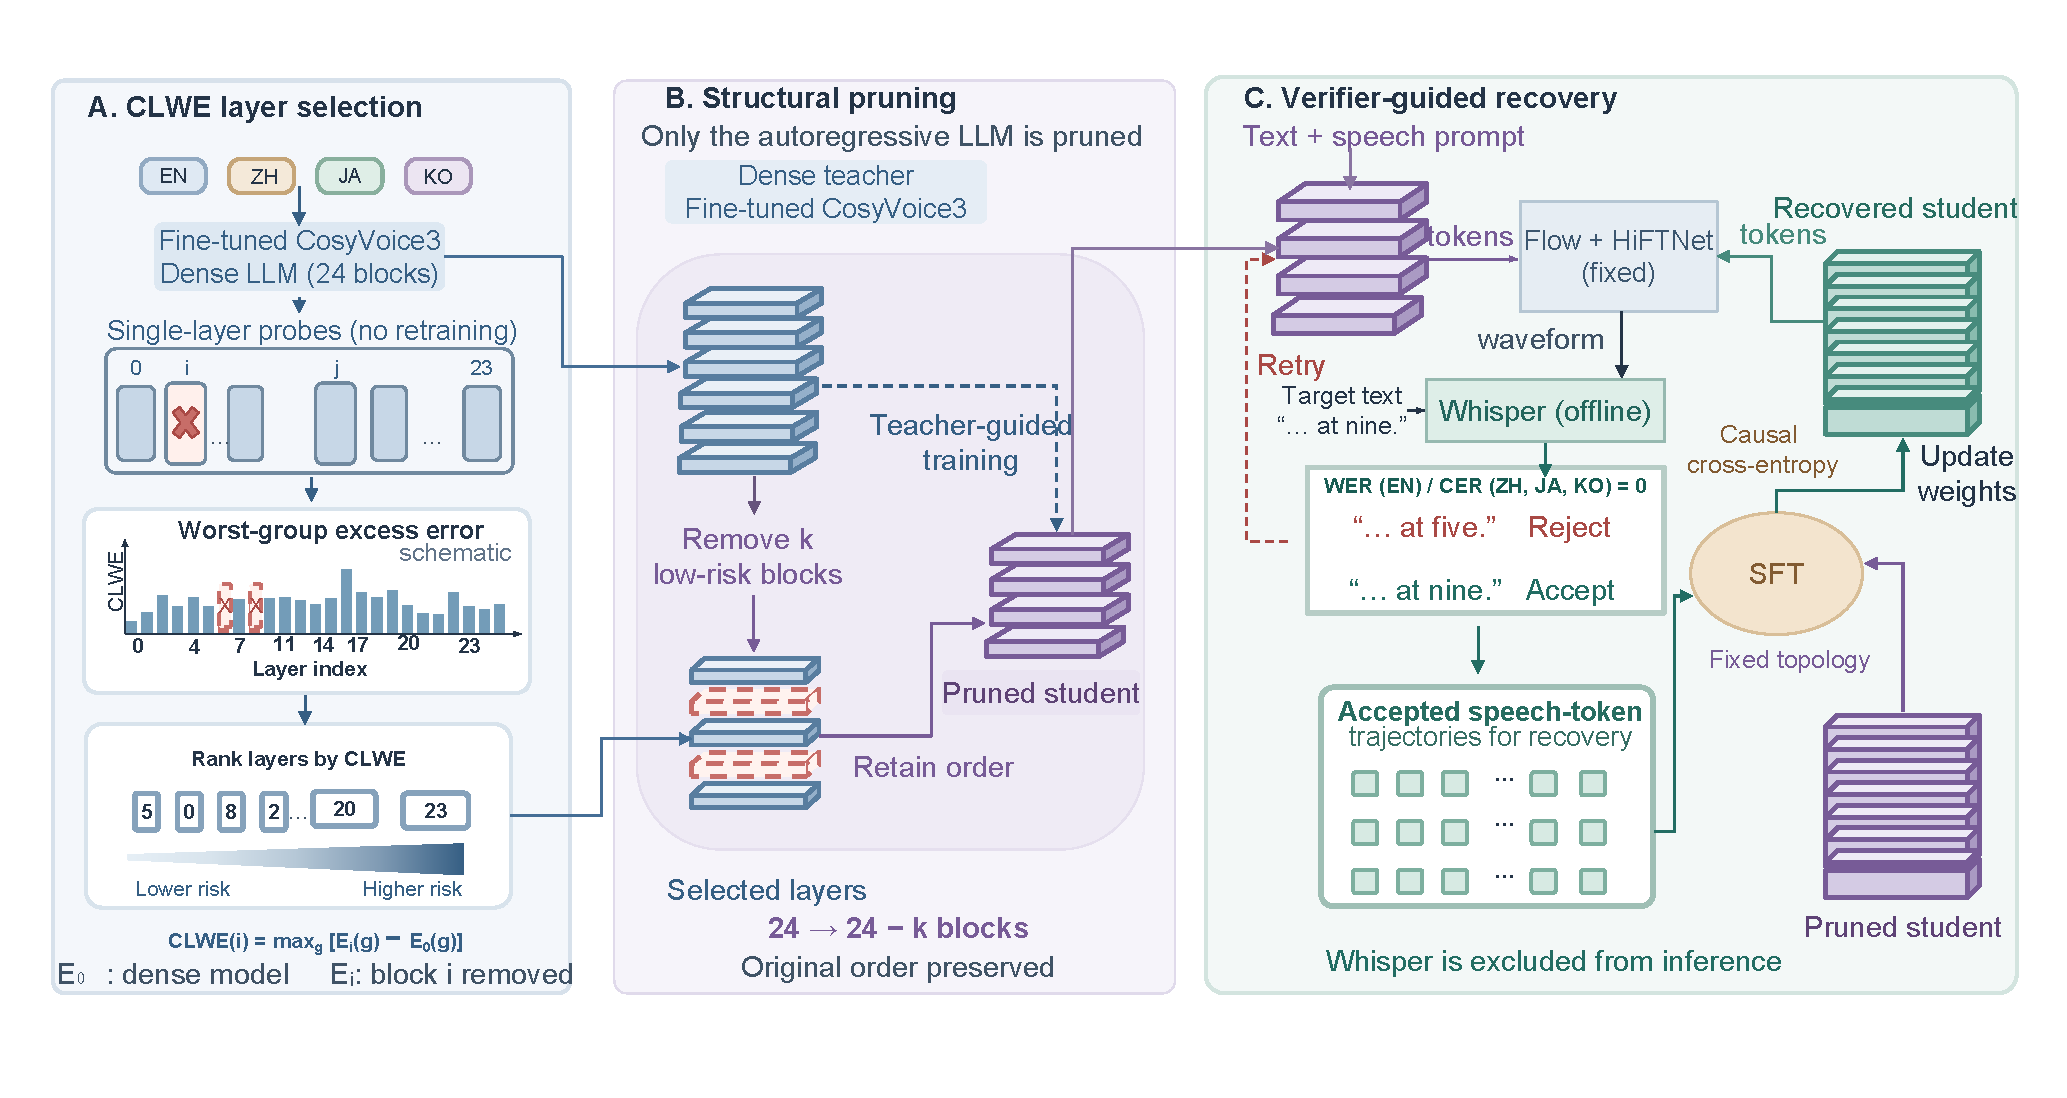
\includegraphics[
width=0.82\textwidth,
keepaspectratio
]{framework.pdf}
\vspace{-2mm}
\caption{Overview of CLWE-Prune. (A) Single-layer-removal experiments
estimate cross-lingual worst-group excess risk. (B) The least important
LLM blocks are physically removed, and post-pruning retraining produces
the Base checkpoint while the acoustic decoder remains fixed. (C) The
pruned student is recovered using speech-token trajectories screened
for content consistency with offline ASR, without changing the pruning
topology.}
\label{fig:framework}
\vspace{-2mm}
\end{figure*}

\section{Method}
\label{sec:method}

Figure~\ref{fig:framework} shows single-layer importance estimation,
structural pruning, and recovery. We rank CosyVoice3's 24
autoregressive LLM blocks, remove the least important ones, and
retrain the pruned model to obtain its Base checkpoint.
The retained blocks inherit Dense-24 weights. In the documented
matched-selection recipe, a frozen Dense-24 teacher guides this
retraining. The lowest-validation-loss checkpoint is selected.
This Base stage precedes the student-trajectory recovery SFT and is
distinct from the Dense-Teacher recovery control.
The flow-matching acoustic model and HiFTNet vocoder remain fixed.

\subsection{CLWE-Based Layer Selection}
\label{sec:clwe_selection}

As illustrated in Fig.~\ref{fig:framework}(A), the calibration set covers
English, Chinese, Japanese, and Korean, using LibriTTS, AISHELL-3,
and Emilia as described in Section~\ref{sec:setup}. Each language is
paired with one corpus domain and has 400 calibration utterances. Thus,
$\mathcal{G}=\{g_{\mathrm{EN}},g_{\mathrm{ZH}},g_{\mathrm{JA}},g_{\mathrm{KO}}\}$
contains four groups. Language and corpus effects are not separated.
For each single-layer removal,
one block $i$ is removed from the Dense model and the remaining network
is evaluated without retraining. All removals follow the same inference
procedure. Let $E_i(g)$ and $E_0(g)$ denote the single-layer-removal
and Dense recognition errors on group $g$, respectively.

Following SPADE's WER-based layer-importance approach
\cite{nguyen2026spade}, the English-only baseline ranks block $i$ by
$R_i^{\mathrm{EN}}=E_i(g_{\mathrm{EN}})$, where $g_{\mathrm{EN}}$ is
the English calibration group. Subtracting the same English baseline
$E_0(g_{\mathrm{EN}})$ from every score leaves this ranking unchanged.
This baseline compares selection criteria rather than reproducing the
full SPADE training pipeline.

CLWE instead defines the group excess error and layer risk as
\begin{equation}
\begin{aligned}
\Delta_i(g) &= E_i(g)-E_0(g), \\
R_i^{\mathrm{CLWE}}
&= \max_{g\in\mathcal{G}} \Delta_i(g),
\end{aligned}
\label{eq:clwe_risk}
\end{equation}
The Dense baseline $E_0(g)$ makes the score relative to each group.
The maximum prevents a severe increase in one group from being masked
by improvements elsewhere. It does not equalize the statistical
properties of English WER and the other languages' CER. Lower scores
indicate safer blocks to remove.

Blocks are ranked in ascending score order, with ties resolved by the
original block index. For a pruning budget of $k$, the first $k$ blocks
are physically removed, as shown in Fig.~\ref{fig:framework}(B). The
ranking is computed once and reused across pruning depths, producing
nested removal sets while preserving the order of retained blocks.
Because single-layer removals do not capture interactions among jointly
removed blocks, this ranking is a heuristic and does not bound the
degradation of the final pruned model.

\subsection{Verifier-Guided Student-Trajectory Recovery}
\label{sec:verifier_recovery}

As shown in Fig.~\ref{fig:framework}(C), each pruned Base model generates
speech-token trajectories $\mathbf{z}=(z_1,\ldots,z_T)$ conditioned on
text $x$ and prompt $p$, with temperature 1.0, top-$p$ 0.8, and
top-$k$ 25. The fixed flow-matching model and HiFTNet
vocoder decode them to speech. After language-specific normalization,
Whisper screens content using WER for English and CER for Chinese,
Japanese, and Korean. Zero-error candidates pass the automatic content
check. Residual ASR mismatches are accepted only after manual content
review. We sample further candidates for unresolved inputs using a
shared reserve text pool when needed. Speaker similarity, UTMOS, and
duration ratio rank candidates after the content check. These scores
do not override it.

For SFT400/15, each pruned Base generates 400 selected targets, and
we report the checkpoint after 15 updates from that Base. For
SFT800/40 at all three depths, we keep these 400 targets and
generate another 400 using an auxiliary checkpoint obtained by
training the same-depth Base on the first set for 60 updates. This
checkpoint only generates additional targets. The final SFT800/40
model starts again from the pruned Base and is trained on all 800
targets for 40 updates.
The ``40'' denotes final-model updates and excludes the auxiliary
student's 60 updates.
For a P12 control, the P12 Base instead generates all 800 targets.
A separate 40-update model also starts from that same Base.
Candidate generation, ASR screening, and auxiliary training are
offline costs, distinct from the inference benchmark.

The accepted trajectories form $\mathcal{D}_{\mathrm{rec}}$. For each
$(x,p,\mathbf{z})\in\mathcal{D}_{\mathrm{rec}}$, we minimize
\begin{equation}
\mathcal{L}_{\mathrm{rec}}
= -\sum_{t=1}^{T}
\log p_{\theta_{\mathrm{P}}}(z_t\mid z_{<t},x,p),
\label{eq:recovery_loss}
\end{equation}
where $\theta_{\mathrm{P}}$ denotes the retained LLM parameters.
Recovery uses a learning rate of $3\times10^{-6}$ and mixed precision.
Teacher forcing increases the likelihood of the accepted token
sequences in the retained LLM. Whisper supplies no training gradients.
% Queue the wide recovery table early enough for a preceding page-top pass.
% Reserve Table 3 while preserving the numbering of the two in-text tables.
\setcounter{savedtablecounter}{\value{table}}
\setcounter{table}{2}
\begin{table*}[!t]
\centering
\caption{Recovery performance and model size on \texttt{strict1200}.
Error rates are percentages. W and SV denote Whisper large-v3 and
SenseVoiceSmall.}
\label{tab:recovery_results}
\small
\setlength{\tabcolsep}{3pt}
\renewcommand{\arraystretch}{1.05}
\begin{tabular}{lcccccccc}
\toprule
\textbf{Recovery Model} & \textbf{W-Macro$\downarrow$} &
\textbf{SV-Macro$\downarrow$} &
\textbf{EN W/SV} & \textbf{ZH W/SV} & \textbf{JA W/SV} &
\textbf{KO W/SV} & \textbf{UTMOS$\uparrow$} & \textbf{MCD$\downarrow$} \\
\midrule
CLWE-Prune P12 (Base) & 8.15 & 9.23 &
2.64/4.11 & 12.36/10.86 & 12.36/14.19 & 5.23/7.76 & 3.4884 & 8.3143 \\
P12 + Verifier-SFT400/15 & 7.53 & 8.40 &
2.61/3.75 & 11.79/10.56 & 11.16/12.41 & 4.58/6.87 & 3.5241 & 8.2449 \\
P12 + Verifier-SFT800/40 & \textbf{7.24} & \textbf{8.32} &
\textbf{2.36}/\textbf{3.68} & 11.51/10.45 & \textbf{10.76}/\textbf{12.39} & \textbf{4.35}/6.74 & \textbf{3.5496} & 8.2541 \\
P12 + Base-Generated-SFT800/40 & 7.62 & 8.33 &
2.55/3.88 & 12.01/10.39 & 11.51/12.40 & 4.39/\textbf{6.64} & 3.5411 & 8.2609 \\
P12 + Selected-Original400/15 & 8.28 & 9.34 &
2.59/4.12 & 12.25/10.71 & 12.50/14.50 & 5.77/8.05 & 3.4746 & 8.2967 \\
P12 + Random-Candidate400/15 & 7.62 & 8.53 &
2.54/3.98 & 12.20/10.67 & 11.33/12.59 & 4.41/6.89 & 3.5133 & \textbf{8.2388} \\
P12 + Dense-Teacher-SFT400/15 & 7.68 & 8.57 &
2.61/4.14 & \textbf{7.16}/\textbf{5.32} & 15.53/16.83 & 5.41/7.99 & 3.5404 & 8.3762 \\
\addlinespace
CLWE-Prune P15 (Base) & 8.91 & 9.73 &
3.00/4.40 & 12.17/10.88 & 13.54/15.07 & 6.94/8.56 & 3.4788 & 8.3662 \\
P15 + Verifier-SFT400/15 & 8.00 & \textbf{8.59} &
2.78/\textbf{4.02} & 12.27/10.78 & 12.39/12.48 & \textbf{4.54}/\textbf{7.08} & 3.5280 & \textbf{8.2871} \\
P15 + Verifier-SFT800/40 & \textbf{7.68} & 8.73 &
\textbf{2.72}/4.24 & 12.09/10.81 & \textbf{11.09}/\textbf{12.44} & 4.83/7.43 & \textbf{3.5543} & 8.2912 \\
P15 + Dense-Teacher-SFT400/15 & 8.82 & 9.44 &
2.93/4.55 & \textbf{7.74}/\textbf{5.81} & 18.72/18.65 & 5.90/8.76 & 3.5282 & 8.4419 \\
\addlinespace
CLWE-Prune P16 (Base) & 9.87 & 10.80 &
3.65/5.30 & 12.69/11.09 & 15.58/17.13 & 7.57/9.69 & 3.4721 & 8.4053 \\
P16 + Verifier-SFT400/15 & 8.82 & 9.50 &
3.38/\textbf{4.54} & 12.35/11.02 & 14.02/14.07 & \textbf{5.54}/8.35 & 3.5345 & 8.3495 \\
P16 + Verifier-SFT800/40 & \textbf{8.32} & \textbf{9.27} &
\textbf{3.21}/4.78 & 12.36/11.12 & \textbf{12.09}/\textbf{13.20} & 5.62/\textbf{7.96} & \textbf{3.5688} & \textbf{8.3476} \\
P16 + Dense-Teacher-SFT400/15 & 10.16 & 10.80 &
3.78/5.28 & \textbf{8.01}/\textbf{6.16} & 21.75/22.44 & 7.08/9.31 & 3.5249 & 8.4836 \\
\addlinespace
Dense-24 Teacher & 7.86 & 8.77 &
2.13/3.39 & 12.21/10.67 & 13.72/14.48 & 3.39/6.52 & 3.4724 & 8.3113 \\
\bottomrule
\end{tabular}%
\vspace{0.5mm}
\parbox{\textwidth}{\small\textit{Note:}
EN uses WER; ZH/JA/KO use CER. Values equally average inference seeds
1986--1988 per fixed checkpoint. Bold marks within-depth best values
(ties included). Dense-24 is a reference. Params (M) counts the full TTS
model, including unchanged acoustic modules: P12/P15/P16 =
680.24/635.50/620.59, and Dense-24 = 859.19. Recovery Base checkpoints
differ from the sweep in Table~\ref{tab:high_compression}.}
\end{table*}
\setcounter{table}{\value{savedtablecounter}}

\section{Experiments and Analysis}
\label{sec:experiments}

\subsection{Experimental Setup}
\label{sec:setup}

\noindent\textbf{Data.}
The calibration set uses 400 utterances per language--corpus group from LibriTTS
(English) \cite{zen2019libritts}, AISHELL-3 (Chinese)
\cite{shi2021aishell3}, and Emilia (Japanese and Korean)
\cite{he2025emilia}. The \texttt{strict1200} test set has 300 utterances
per language. Models share test texts and prompts but generate separate
waveforms. Recovery uses 100 or 200 targets per language for
SFT400/15 or SFT800/40.


\noindent\textbf{Models and training configurations.}
Dense-24 is unpruned. P$k$ removes $k$ LLM blocks, and Base precedes
recovery. English-WER and CLWE-Prune use matched post-pruning retraining,
lowest-loss selection, and evaluation at P6--P12. Tables~\ref{tab:criterion_comparison}
and~\ref{tab:high_compression} use inference seed 1986. The latter is
an exploratory P13--P17 CLWE configuration sweep.

Table~\ref{tab:recovery_results} evaluates P12, P15, and P16 Base
checkpoints from a branch separate from the sweep. Both recovery
budgets cover all three depths. The 400/15 controls use original
recording tokens (Selected-Original, P12), unverified student targets
with separately assigned same-language prompts (Random-Candidate,
P12), or verified dense targets (Dense-Teacher, all depths).

\noindent\textbf{Evaluation metrics.}
Content accuracy is evaluated using Whisper large-v3
\cite{radford2023whisper} and SenseVoiceSmall
\cite{an2024funaudiollm}. WER is used for English, while CER is used for Chinese,
Japanese, and Korean. We report macro-averaged error rate (Macro ER),
computed as the mean of the four language-level error rates.
Table~\ref{tab:recovery_results} averages decoding seeds 1986--1988
per fixed checkpoint, not training runs. Changes use unrounded values.
For a model
evaluated alongside Dense-24, the test worst-group excess is
$\max_g[E_{\rm model}(g)-E_{\rm Dense}(g)]$.

We report UTMOS predicted quality \cite{saeki2022utmos} and
mel-cepstral distortion (MCD) in the recovery comparison. The
high-compression sweep also reports CAM++ speaker embedding cosine
similarity (SECS) \cite{wang2023campp}. MCD uses 24-kHz WORLD
24-order mel cepstra (excluding $c_0$) aligned with fastDTW.
Higher UTMOS/SECS and lower MCD are preferred. UTMOS also ranks
candidates, and automatic scores do not establish perceived naturalness.
A separate architecture benchmark measures
streaming real-time factor (RTF, synthesis time divided by audio
duration), first-packet latency, and peak allocated CUDA memory.

\par\smallskip
\noindent\begin{minipage}{\columnwidth}
\centering
\captionof{table}{English-WER versus CLWE layer selection. Error rates are
percentages.}
\label{tab:criterion_comparison}
\small
\setlength{\tabcolsep}{1.0pt}
\renewcommand{\arraystretch}{1.05}
\begin{tabular}{lcccc}
\toprule
\textbf{Model} &
\textbf{Macro$\downarrow$} &
\textbf{EN/ZH$\downarrow$} &
\textbf{JA/KO$\downarrow$} &
\textbf{UTMOS$\uparrow$/MCD$\downarrow$} \\
\midrule
EN-WER P6 & 7.92 & 2.16/12.17 & 12.12/5.26 & 3.47/8.32 \\
CLWE P6 & \textbf{7.67} & 2.75/\textbf{11.67} & \textbf{11.92}/\textbf{4.34} & \textbf{3.48}/\textbf{8.28} \\
EN-WER P8 & 7.91 & 2.23/12.67 & 11.93/4.81 & 3.47/8.32 \\
CLWE P8 & \textbf{7.65} & \textbf{2.04}/\textbf{12.01} & 12.16/\textbf{4.37} & \textbf{3.48}/\textbf{8.26} \\
EN-WER P10 & 8.47 & 2.81/11.97 & 13.85/5.27 & 3.48/8.27 \\
CLWE P10 & \textbf{7.78} & \textbf{2.53}/12.28 & \textbf{11.45}/\textbf{4.88} & 3.47/8.29 \\
EN-WER P12 & 8.97 & 2.64/12.10 & 16.25/4.90 & 3.49/8.31 \\
CLWE P12 & \textbf{8.09} & \textbf{2.42}/12.38 & \textbf{12.51}/5.04 & 3.48/8.32 \\
\bottomrule
\end{tabular}%

\vspace{0.5mm}
\parbox{\columnwidth}{%
\small
\textit{Note:}
EN reports WER; ZH, JA, and KO report CER.
Bold indicates metrics for which CLWE-Prune outperforms English-WER
at the same pruning depth.
}
\end{minipage}\par\smallskip

\subsection{Results and Analysis}
\label{sec:results}

\par\smallskip
\noindent\begin{minipage}{\columnwidth}
\centering
\captionof{table}{High-compression quality sweep and separate architecture
inference benchmark. L denotes retained blocks. Macro ER is Whisper
Macro ER (\%).}
\label{tab:high_compression}
\small
\setlength{\tabcolsep}{2.5pt}
\renewcommand{\arraystretch}{1.05}
\begin{tabular}{lccccc}
\toprule
\textbf{Model} & \textbf{Layers} & \textbf{Macro ER$\downarrow$} &
\textbf{UTMOS$\uparrow$} & \textbf{SECS$\uparrow$} &
\textbf{MCD$\downarrow$} \\
\midrule
CLWE P13 & 11 & 8.36 & 3.48 & 0.80 & 8.31 \\
CLWE P14 & 10 & 8.65 & 3.48 & 0.80 & 8.36 \\
CLWE P15 & 9  & 8.75 & 3.48 & 0.80 & 8.35 \\
CLWE P16 & 8  & 11.31 & 3.47 & 0.80 & 8.40 \\
CLWE P17 & 7  & 13.17 & 3.48 & 0.80 & 8.46 \\
\bottomrule
\end{tabular}%
\vspace{0.6mm}

\begin{tabular}{lcccc}
\toprule
\textbf{Architecture} & \textbf{L} & \textbf{RTF$\downarrow$} &
\textbf{First packet (s)$\downarrow$} & \textbf{Peak CUDA (MiB)$\downarrow$} \\
\midrule
Dense-24 & 24 & 0.633 & 2.600 & 3382 \\
12-layer & 12 & 0.434 & 1.779 & 2697 \\
9-layer & 9 & 0.375 & 1.572 & 2530 \\
8-layer & 8 & 0.377 & 1.535 & 2468 \\
\bottomrule
\end{tabular}%
\vspace{0.4mm}
\parbox{\columnwidth}{\small\textit{Note:}
RTX 3090, FP32, batch size 1, 30 English utterances, three repeats.
Peak CUDA is mean per-sample allocated memory. Efficiency checkpoints
differ from the quality sweep and Table~\ref{tab:recovery_results}.}
\end{minipage}\par\smallskip
\setcounter{table}{3} % Tables 1--3 have now been numbered.


Table~\ref{tab:criterion_comparison} compares layer rankings at
matched depths. CLWE lowers Whisper Macro ER by 0.25, 0.26, 0.69, and
0.88 points at P6, P8, P10, and P12. The largest reported language
error also falls by 0.25, 0.51, 1.57, and 3.74 points, respectively.
This descriptive maximum mixes English WER with the other languages'
CER. P12 Japanese CER (16.25\% to 12.51\%) shows the non-English
regression missed by English-only ranking. P10 Chinese CER rises by
0.31 points, so gains are not uniform. Mean-Excess and Max-Raw
checkpoints were not evaluated, so this comparison does not isolate
the maximum operation or Dense-baseline subtraction. The matched
comparison ends at P12.

Table~\ref{tab:high_compression} reports available CLWE configurations,
not a controlled depth-only ablation. Whisper Macro ER rises from
8.36\% at P13 to 8.75\% at P15 and 11.31\% at P16, while UTMOS and
SECS barely change. This motivates testing recovery at nine and eight
layers. In the separate architecture benchmark, RTF falls from 0.633
for Dense-24 to 0.375 for nine layers (1.69$\times$). First-packet
latency falls from 2.600 to 1.572 s. These efficiency checkpoints
are distinct from the quality and recovery checkpoints. Peak allocated
CUDA memory falls from 3382 to 2530 MiB. The eight-layer architecture
has a slightly lower first-packet latency (1.535 s) but no further RTF
gain (0.377). The measured quality and efficiency trends favor nine
layers among these configurations.

Relative to their respective Base models in
Table~\ref{tab:recovery_results}, Verifier-SFT400/15 reduces
Whisper/SenseVoice Macro ER by 0.62/0.83, 0.92/1.14, and 1.05/1.31
points at P12, P15, and P16, respectively. UTMOS increases and MCD
decreases at each depth without changing parameter counts. SenseVoice
does not select targets, so its improvement supports a content gain
beyond the Whisper screening metric. Among 24 per-language ASR values
(three depths, four languages, two recognizers), 23 decrease. The sole
exception is P15 Chinese Whisper CER (12.17\% to 12.27\%). This breadth
shows that the macro gains are not driven by one language. UTMOS also
ranks accepted targets.
SFT800/40 further improves both ASR measures at P12 and P16. At P15,
Whisper improves from 8.00 to 7.68 but SenseVoice rises from 8.59 to
8.73. Relative to their own Base checkpoints, the P15 and P16
SFT800/40 models reduce Whisper/SenseVoice Macro ER by 1.23/1.00 and
1.55/1.54 points. At P15, UTMOS increases from 3.4788 to 3.5543 and
MCD decreases from 8.3662 to 8.2912. These automatic acoustic scores
move with the recognition gains, although UTMOS is also used to rank
accepted recovery candidates.
The recovered nine-layer model has 635.50M total parameters,
versus 859.19M for Dense-24, and observed Macro ER of 7.68/8.73
versus 7.86/8.77. Its worst-group Whisper excess over Dense-24 is
still 1.44 points in Korean (4.83 versus 3.39). English WER is also
0.59 points higher. Thus, the lower macro average does not imply
uniform language-level preservation.

At P12, Selected-Original is slightly worse than Base (8.28/9.34
versus 8.15/9.23), while Random-Candidate reaches 7.62/8.53 and
verified student recovery reaches 7.53/8.40. Student-generated targets
give the larger observed gain, consistent with the on-policy rationale
\cite{agarwal2024onpolicy}. Different prompts prevent assigning the
smaller verified--random gap solely to ASR screening.
With 800 targets, mixed Base/auxiliary generation reaches 7.24/8.32
versus 7.62/8.33 when Base generates all targets, with separate
training runs. Dense-Teacher at P15 lowers Chinese Whisper CER from
12.17\% to 7.74\% but raises Japanese CER from 13.54\% to 18.72\%.
At the same 400-target/15-update setting, verified student targets
yield lower Whisper/SenseVoice Macro ER than Dense-Teacher targets by
0.15/0.17, 0.82/0.85, and 1.33/1.30 points at P12, P15, and P16.
The Japanese Whisper CER gap is especially large at P15 (12.39\%
versus 18.72\%) and P16 (14.02\% versus 21.75\%), whereas the
teacher targets improve Chinese. Thus the lower macro errors do not
merely reflect a single favorable language. These fixed-checkpoint
results support student-specific targets but do not isolate the
mechanism or quantify training variability.

\section{Conclusion}
\label{sec:conclusion}

CLWE-Prune lowers Whisper Macro ER against English-only selection at
four tested depths. P12 Japanese CER falls by 3.74 points. Student
trajectory recovery improves both ASR measures at P12, P15, and P16
without restoring layers. The recovered nine-layer model uses 26.03\%
fewer parameters than Dense-24 and has slightly lower observed macro
errors, although English and Korean errors remain higher. A separate
architecture benchmark measures a 1.69$\times$ streaming RTF speedup.

\section{Compliance with Ethical Standards}
This study used existing publicly available speech corpora and
involved no new data collection or interaction with human
participants. No additional ethical approval was required.

% Before submission, add an Acknowledgment section here after the
% authors confirm funding, competing interests, and generative-AI use.

% uncomment the preceding line ``\centerline...'' and replace ``imageX.ps''
% with a suitable PostScript file name.
% -------------------------------------------------------------------------




% References should be produced using the bibtex program from suitable
% BiBTeX files (here: strings, refs, manuals). The IEEEbib.bst bibliography
% style file from IEEE produces unsorted bibliography list.
% -------------------------------------------------------------------------
\bibliographystyle{IEEEbib}
\begingroup\small
\bibliography{refs}
\endgroup

\end{document}
